\documentclass[tikz,border=10pt]{standalone}
\usetikzlibrary{decorations.markings,arrows.meta}

\begin{document}
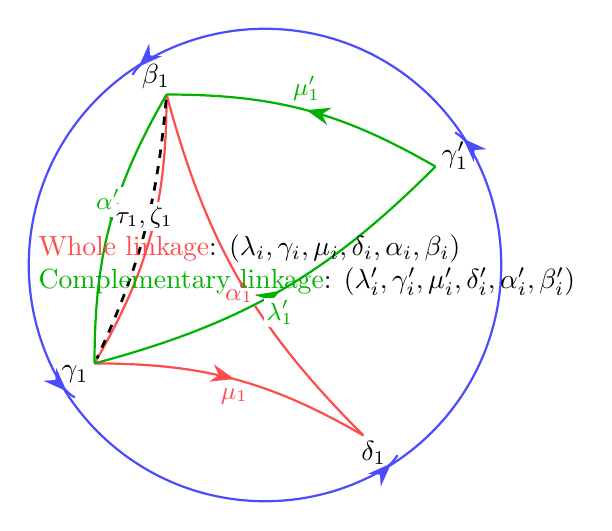
\begin{tikzpicture}[
    sphere/.style = {circle, draw=blue!70, thick, minimum size=6cm},
    arc/.style = {decoration={markings, mark=at position 0.5 with {\arrow{Stealth[length=3mm]}}},
                  postaction={decorate}, thick},
    gap/.style = {dashed, line width=1pt, shorten >=2pt, shorten <=2pt},
    label/.style = {font=\small, fill=white, inner sep=1pt}
]
    % Sphere
    \node[sphere] (sphere) at (0,0) {};
    
    % Spherical triangle vertices
    \coordinate (A) at (120:2.5);
    \coordinate (B) at (210:2.5);
    \coordinate (C) at (300:2.5);
    \coordinate (D) at (30:2.5);
    
    % First linkage (whole)
    \draw[arc, red!70] (A) to[bend left=15] node[label,above=2pt] {$\lambda_1$} (B);
    \draw[arc, red!70] (B) to[bend left=15] node[label,below=2pt] {$\mu_1$} (C);
    \draw[arc, red!70] (C) to[bend left=15] node[label,below=2pt] {$\alpha_1$} (A);
    
    % Second linkage (complementary)
    \draw[arc, green!70!black] (B) to[bend right=15] node[label,below=2pt] {$\lambda'_1$} (D);
    \draw[arc, green!70!black] (D) to[bend right=15] node[label,above=2pt] {$\mu'_1$} (A);
    \draw[arc, green!70!black] (A) to[bend right=15] node[label,above=2pt] {$\alpha'_1$} (B);
    
    % Angle markers
    \foreach \point/\angle/\param in {
        A/120/{$\beta_1$},
        B/210/{$\gamma_1$},
        C/300/{$\delta_1$},
        D/30/{$\gamma'_1$}} {
        \draw[arc, blue!70] (\point) +(\angle:0.5cm) arc(\angle:\angle+30:0.5cm);
        \node at (\point) [anchor=\angle+180, inner sep=2pt] {\param};
    }
    
    % Gap between beta_1 and alpha_2
    \draw[gap] (A) to[bend left=10] node[label,above] {$\tau_1, \zeta_1$} (B);
    
    % Legend
    \node[align=left, anchor=west] at (-3,0) {
        \textcolor{red!70}{Whole linkage}: $(\lambda_i, \gamma_i, \mu_i, \delta_i, \alpha_i, \beta_i)$\\
        \textcolor{green!70!black}{Complementary linkage}: $(\lambda'_i, \gamma'_i, \mu'_i, \delta'_i, \alpha'_i, \beta'_i)$
    };
\end{tikzpicture}
\end{document}